\newpage{}

\section{Simulation Analysis}
\label{sec:simulation}
\paragraph{}


\par In this part of the report, the NGSpice results for the same analysis as the theoretical will be presented. The purpose of it was to obtain the best possible value for gain, lower and upper cutoff frequencies and bandwidth in order to maximize the merit. We followed a set of steps as follows:
\begin{itemize}
	\item First, we used the Phillips transistor model provided by the professor to design the circuit.
	\item Then, we had to verify that the transistor operation was in the forward active region (F.A.R mode).
\end{itemize}

\begin{table}[H]
  \centering
  \begin{tabular}{|c|c|}
    \hline    
    \input{../sim/pnp_TAB.tex}
  \end{tabular}
  \caption{Verification F.A.R. mode for the PNP transistor}
  \label{sim1}
\end{table}

\begin{table}[H]
  \centering
  \begin{tabular}{|c|c|}
    \hline    
    \input{../sim/npn_TAB.tex}
  \end{tabular}
  \caption{Verification F.A.R. mode for the NPN transistor}
  \label{sim1}
\end{table}

\begin{itemize}
	\item Afterwards, we computed the currents and nodal voltages for the Output Circuit.
	\item With that, we measured the output voltage gain, lower and upper cutoff frequencies and the bandwidth in the array of values for frequency, obtaining the following values:
\end{itemize}

\begin{table}[H]
  \centering
  \begin{tabular}{|c|c|}
    \hline    
    \input{../sim/results_TAB.tex}
  \end{tabular}
  \caption{Results obtained in NgSpice}
  \label{sim1}
\end{table}


\par With these values, we were able to draw some conclusions on the components of this circuit:
\par \textbf{Coupling Capacitors}
\par These components are tasked with blocking DC signals. In an amplifier specifically, constant values must be eliminated which is why they are used. However, they also come with the cost of blocking some lower frequencies, which affects the bandwidth.
\par \textbf{Bypass Capacitor}
\par In this circuit, the existence a Re resistor to bridge the effect of temperature of DC current passing through it, which comes at the cost of gain reduction, calls for the need of a bypass capacitor, placed in parallel to the previously mentioned resistor so that DC current continues being affected by it while AC current bypasses it completely, not affecting the gain.
\par \textbf{RC Resistor}
\par This component is placed in the circuit with the objective of increasing the gain. 
\par The importance of these components can be seen by the effects they have on the graphics below:

\begin{figure}[H]
    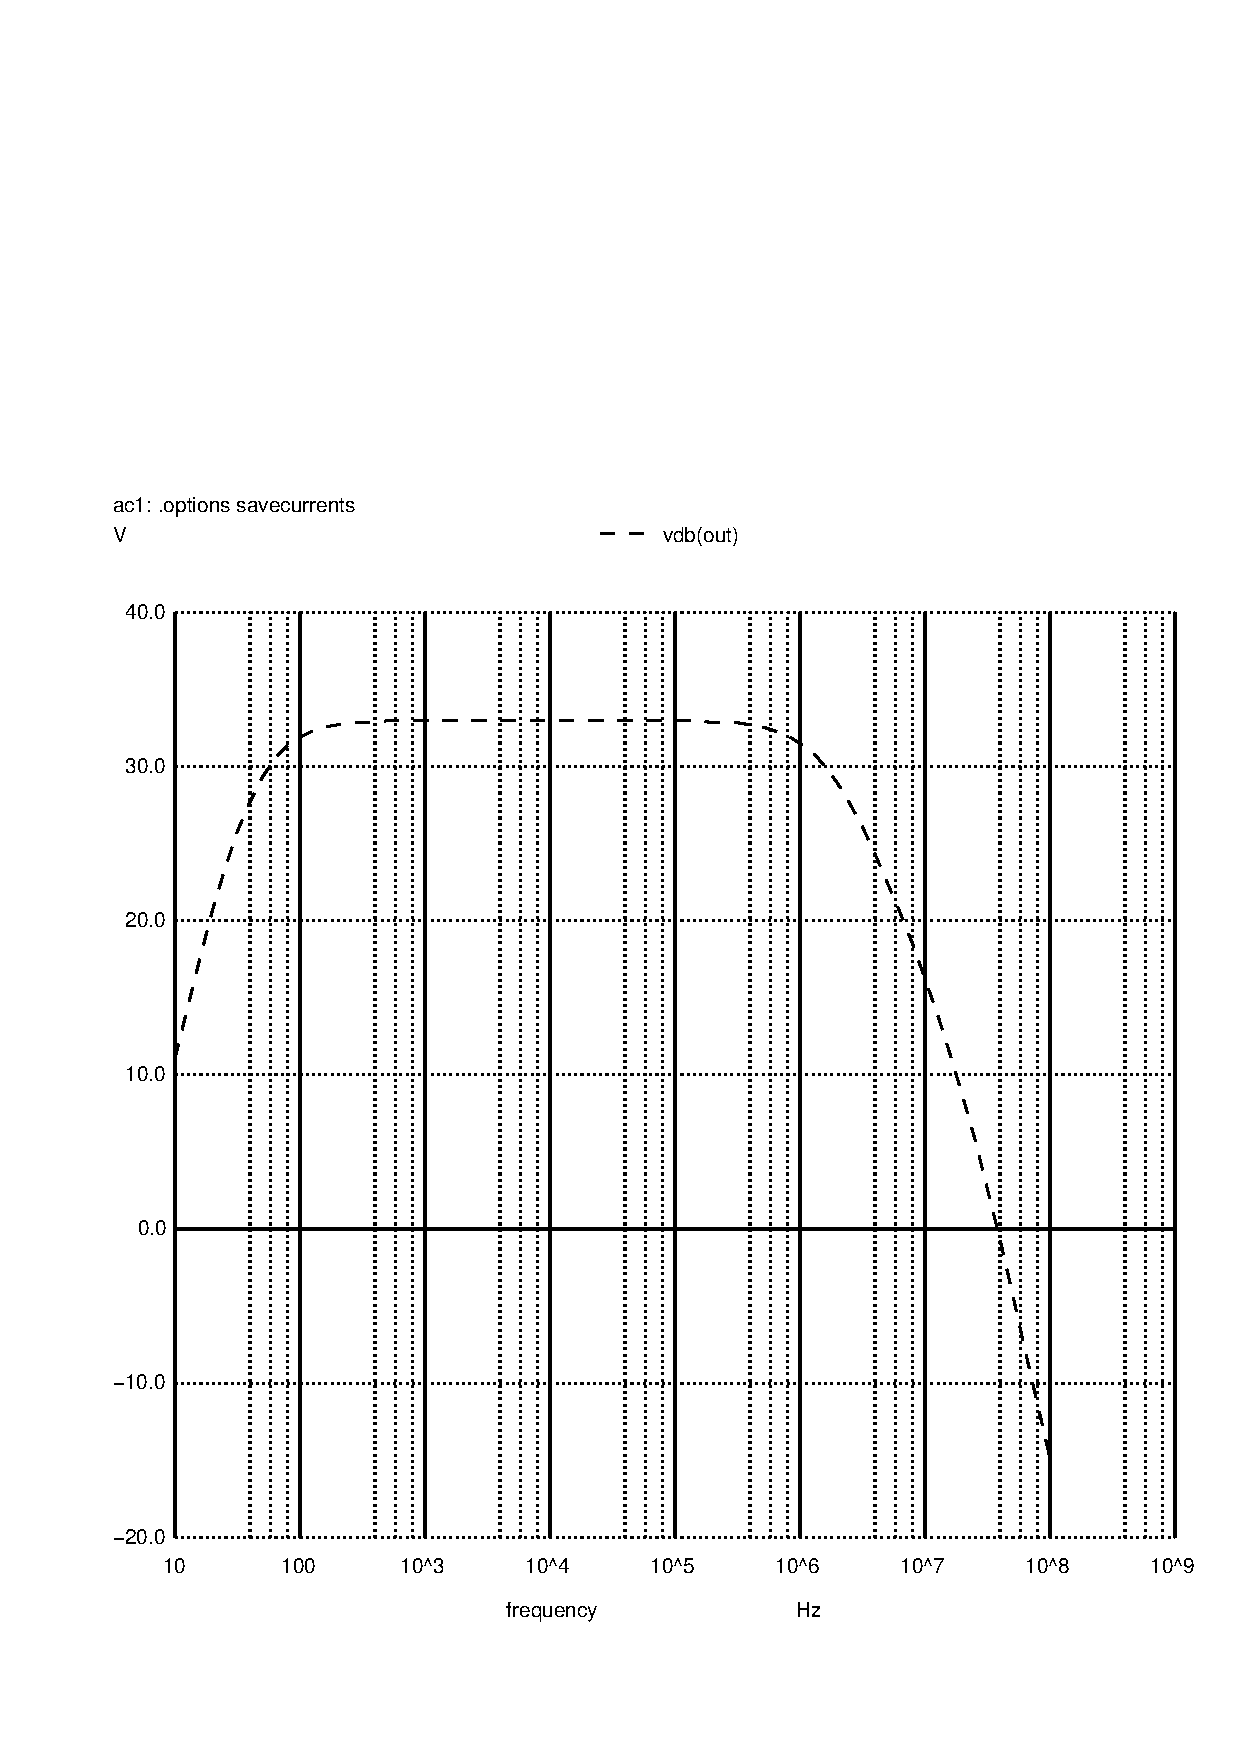
\includegraphics[width=0.495\linewidth]{../sim/vo2f.pdf}
    \centering
    \caption{$v_0-12$ (Deviation from the desired DC voltages)}
    \label{mag}
\end{figure}

\begin{itemize}
	\item After all that, we determined the Input impedance:
\end{itemize}

\begin{table}[H]
  \centering
  \begin{tabular}{|c|c|}
    \hline    
    \input{../sim/zin_TAB.tex}
  \end{tabular}
  \caption{Input impedance}
  \label{sim1}
\end{table}

\begin{itemize}
	\item And then the Output impedance:
\end{itemize}

\begin{table}[H]
  \centering
  \begin{tabular}{|c|c|}
    \hline    
    \input{../sim/zout_TAB.tex}
  \end{tabular}
  \caption{Output impedance}
  \label{sim1}
\end{table}


\begin{itemize}
	\item Lastly, we were able to figure out whether or not the amplifier is efficient by calculating the cost and merit from the equation shown in the Introduction:
\end{itemize}

\begin{table}[H]
  \centering
  \begin{tabular}{|c|c|}
    \hline    
    \input{../sim/merit_TAB.tex}
  \end{tabular}
  \caption{Merit}
  \label{sim1}
\end{table}
